\documentclass[11pt, a4paper]{jreport}

\usepackage[driver=dvipdfm]{geometry}
\usepackage[dvipdfmx]{graphicx, color}
\usepackage{here}
\usepackage{plext}
\usepackage{times, mathptmx}
\usepackage{longtable}
\usepackage{colortbl}
\usepackage{tabularx}
\usepackage{enumerate}
\usepackage{comment}
\usepackage{url}
\usepackage{lscape}
\usepackage{multirow}
%\usepackage{otf}

\setlength{\voffset}{0.5truecm}
\setlength{\headsep}{2truecm}
\setlength{\oddsidemargin}{7.0truemm}
\setlength{\evensidemargin}{-5.5truemm}
\setlength{\topmargin}{-1truecm}
\setlength{\footskip}{25truemm}
\setlength{\textwidth}{15truecm}
\setlength{\textheight}{22truecm}
\makeatletter
\makeatother

\begin{document}
    \title{プログラムコードの複雑さの防止効果が高い\\システム開発上の要素の検討\\Consideration of view points\\that contribute to the prevention of\\program code complexity in system development}
    \author{指導教員:山川 広人\\
    公立 千歳科学技術大学 理工学部\\
    情報システム学科 山川研究室\\
B2201400 須藤 真由}
\date{\today}

\maketitle
\pagenumbering{roman}
\tableofcontents
\chapter{序論}
\pagenumbering{arabic}

\section{背景}
プログラムコードにおける認知負荷に注目が集まっている.平嶋ら\cite{haikei}は高等教育機関におけるプログラミング講義に苦手意識を持つ学習者に着目し,プログラミング学習者の認知負荷を減少させ、アルゴリズムの組み立て等の適切な部分に認知資源を集中させるべきだと述べている。社会的にもプログラムコードの認知負荷に対する取り組みや議論は盛んである。オープンワーク株式会社ではエンジニアによるブログで認知負荷を低減するために実践している事例を公開している。株式会社カケハシとリクルートホールディングスが合同で開催したイベントでの講演では、実際に直面したシステム開発中の課題の1つとして認知負荷の増大を挙げていた。認知負荷が高い状態は学習やシステム開発をする上で問題となり、システムの継続的な発展のためにも解決すべき課題であると捉えられている。
\\ 認知負荷に対する研究は高等教育機関におけるPBL学習(Ploject Based Learning)に対しても有用である。PBL学習には企業や地域のステークホルダーと連携し、数世代に亘ってプロジェクトを引継ぐことで成果物の発展や価値提供を行い続けるものがある。しかし、複雑さを招かずにシステム開発をする知識や認知負荷を下げるという意識を学生が必ずしも持ち合わせてはいないので、成果物として複雑なプログラムコードが出来上がることがある。その成果物を次の世代のプロジェクトが引き継ぐ際に、複雑なプログラムコードを読み解くことに時間がかかり問題解決に認知資源を集中できないことや、新たにプログラムコードを追加、変更した際に、さらに複雑なものにしてしまうことがある。PBL学習を効果的に行うためにも、複雑さの原因や複雑さを防止する方法について明らかにする必要がある。

\section{目的}
本研究ではステークホルダーと継続的に価値共創を行っていくシステム開発プロジェクトを想定し、複雑さが防止されたプログラムコードの設計、開発方法を明らかにすることが目的である。プログラムコードの複雑さが招かれる原因ははどこに存在しているかを分析し、どのような要素を取り入れることで複雑さを防止できるか、また複雑さが防止できていることをどのように確認できるか検討することで以下に示す2点のリサーチクエスチョンについて検証し、検討した要素や方法の有用性について考察を行う。
\begin{itemize}
\item プログラムコードの複雑さの防止効果が高いシステム開発上の要素は何か
\item その要素がプログラムコードに
反映されているか評価する方法は何か
\end{itemize}
\section{構成}

\chapter{先行研究と本研究の位置づけ}
\section{先行研究}
\subsection{}
\subsection{}
\section{本研究の位置づけ}
\chapter{複雑さの原因の分析と改善案の提案}
\section{複雑さの原因の分析}
プログラムコードの複雑さを招いている現状を分析し、複雑さの原因を分析する。複雑化したプログラムコードとして公立千歳科学技術大学で開発が進められてきた既存のシステムである「話しことばチェッカー」のプログラムコードを用いる。このシステムは文章を入力し検出ボタンを押すと文章内から話しことばを検出し、修正例と共に検出結果を示す文章校正システムである。プログラムコードを読み複雑さの原因となる問題点を洗い出したところ、以下の3つの状態になっていたことが複雑さの原因であると判明した。
\begin{enumerate}
\item どのような役割がどこに書かれているのか分からないコード
\item 開発者の独自の解釈を反映させたコード
\item どのような操作でどのような結果を示すのか分からないコード
\end{enumerate}
 1について、以下に示した図3.1のプログラムコードのように1つのメソッドに多くの役割が含まれていること、話しことばの検出にまつわるメソッドがまとめて1つのクラスに書かれており、検出についての詳細な処理がどこに書かれているか探しにくい状態になっていた。
\begin{figure}[H]
\centering 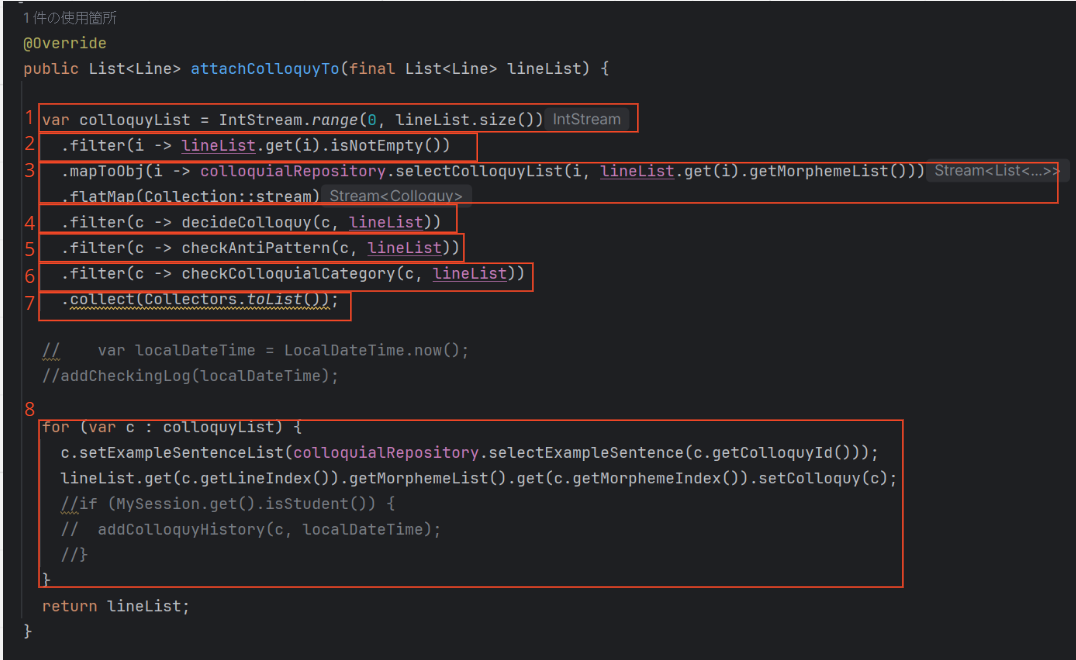
\includegraphics[width=1\linewidth]{image/genin1.1.png}
\caption{どのような役割がどこに書かれているのか分からないコードの例}
\label{fig:enter-label}
\end{figure}
 2について、話しことばの検出の過程には形態素解析を行った後に形態素の前後関係を用いるものがあり、それらをカテゴリで分類し判断している。その中で、下に示す図3.2のクラス構造の赤丸で示したようにいくつか前の形態素を用いるものを"C2"や"Prefix"、「1つ」、「2つ」、「3つ」をドイツ語で"Eins"、"Zwei"、"Drei"等のように開発者独自の命名でプログラムコード上に示している。こういった命名や他にも処理の内容や順番に開発者独自の考えが反映されていた。
\begin{figure}[H]
\centering
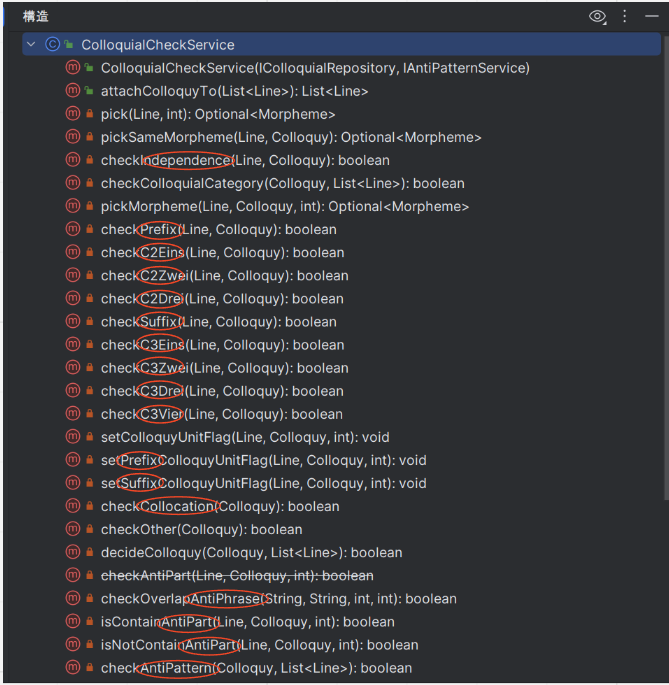
\includegraphics[width=1\linewidth]{image/genin2.1.png}
\caption{開発者の独自の解釈を反映させたコードの例}
\label{fig:enter-label}
\end{figure}
 3について、このシステムがどのような操作でどのような結果を示すものなのか、どのような実装がされていればステークホルダーの要求を満たしているのか、確かめる手段が用意されていなかった。
\section{複雑さの防止方法の提案}
プログラムコードの複雑さの原因に基づき、ドメイン駆動設計やテスト駆動開発で使用される方法を用いてリファクタリングを行いプログラムコードの改善を行う。
\subsection{ドメイン駆動設計}
ドメイン駆動設計はドメインモデルに従って設計を行う設計手法であるため、どのような役割がどこに書かれているのか分からないコードとなっている部分と開発者の独自の解釈を反映させたコードとなっている部分の改善に有効であると想定している。
\subsection{テスト駆動開発}
テスト駆動開発は満たすべき要件を実装前にテストコードとして書く開発手法である。テストコードを書くことでどのような操作でどのような結果を示すのか分からないコードの改善を狙っている。
\chapter{リファクタリングによるコードの改善}
\section{改善方法}
\subsection{モデリング}
ドメイン駆動設計の手法を用いてモデリングを見直す。ドメイン駆動設計ではドメインモデルを通じて機能を実装する。本研究では話しことばチェッカーの共同研究者でありドメインに深く通じている山下の論文からドメインモデルを吸い上げモデリングに使用する。またモデリングや実装の際の命名もドメインモデルから吸い上げたユビキタス言語を使用する。
\subsection{テストコードの作成}
このシステムが何をするのか、観察可能な振る舞いの考えをもとに単体テストとして書き起こす。テスト駆動開発を取り入れ、モデリングで整理した満たすべき要件をリファクタリング前と結果を変えずに実装できているようにする。テストコードにもモデリングと同様にユビキタス言語を使用する。
\section{改善結果}
リファクタリングを経て、以下のように複雑さの原因を含んだプログラムコードを複雑さが解消されたプログラムコードに改善できた。
\begin{enumerate}
\item どのような役割がどこに書かれているのか分からないコードを、責務を分けたコードに改善
\item 開発者の独自の解釈を反映させたコードを、共有されたメンタルモデルを反映したコードに改善
\item どのような操作でどのような結果を示すのか分からないコードを、観察可能な振る舞いが確認できるコードに改善
\end{enumerate}
 1について、元のプログラムコードは下に示す図4.1の赤い矢印より左のようなアーキテクチャであり、Service層に細やかな役割のことである責務が集中していた。モデリングを行ったことにより赤い矢印より右のようなアーキテクチャへと変化した。Domain層に計算・加工・判断など話しことば検出に必要な責務を分離し、どこにどの責務があるのか、明確になった。
\begin{figure}[H]
\centering
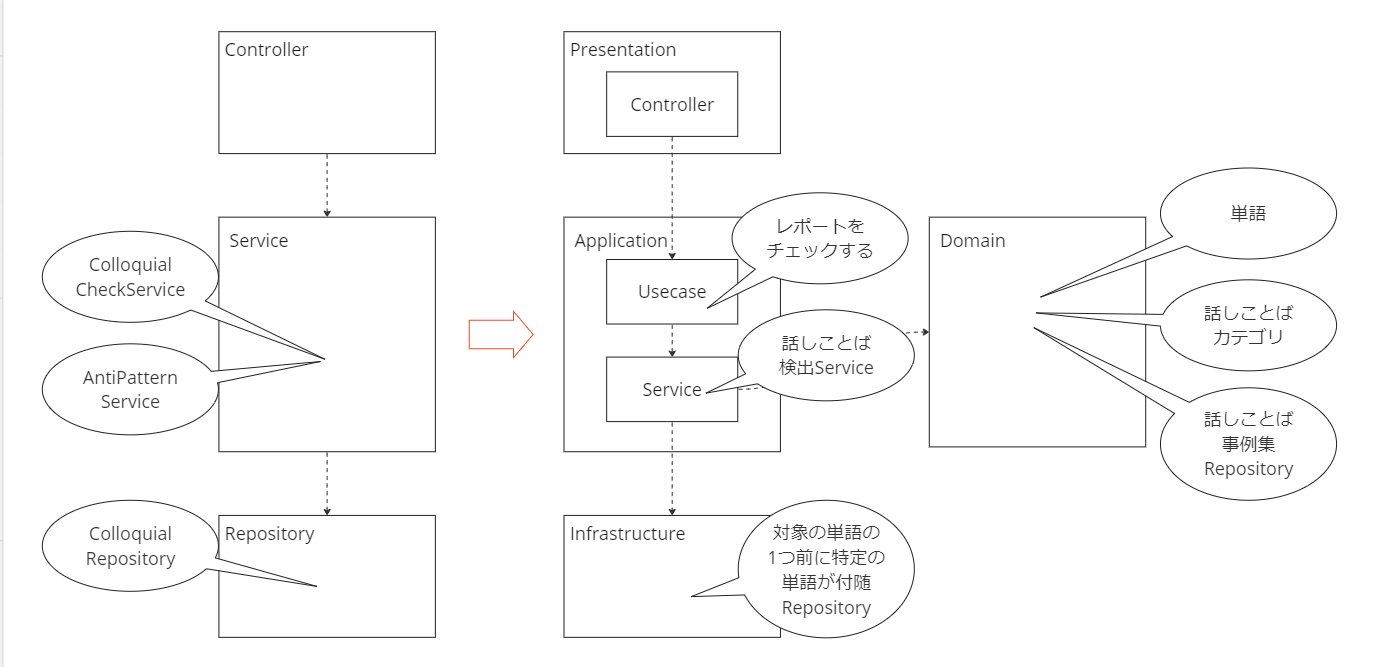
\includegraphics[width=1\linewidth]{image/kaizen1.png}
\caption{リファクタリングによるアーキテクチャの変化}
\label{fig:enter-label}
\end{figure}
 2について、山下の論文内に存在する語をユビキタス言語として使用し、下に示す図4.2のように日本語の単位をモデリングに取り入れたことで、問題の解決方法の解釈のことであるメンタルモデルをプログラムコードに反映した。それにより、命名や構造に開発者の独自の解釈を用いていないプログラムコードへと改善した。
\begin{figure}[H]
\centering
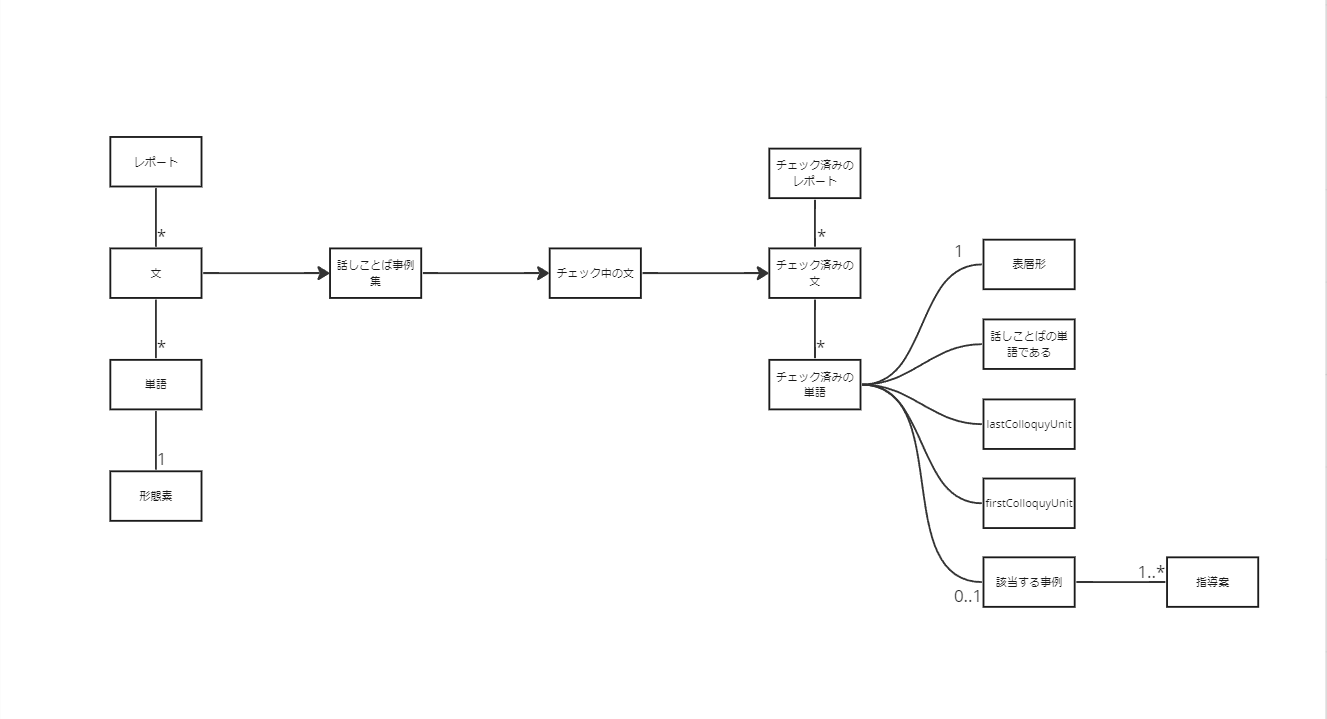
\includegraphics[width=1\linewidth]{image/kaizen2.png}
\caption{プログラムコードに反映したメンタルモデルの一部}
\label{fig:enter-label}
\end{figure}
 3について、プログラムコードにテストコードを追加したことで、このシステムではどのような操作と結果が期待されているのか確認できるようになった。下の図4.3に示すようにテストケースの命名、入力と期待する出力にこういった観察可能な振る舞いを確認することができるようなプログラムコードに改善した。
\begin{figure}[H]
\centering
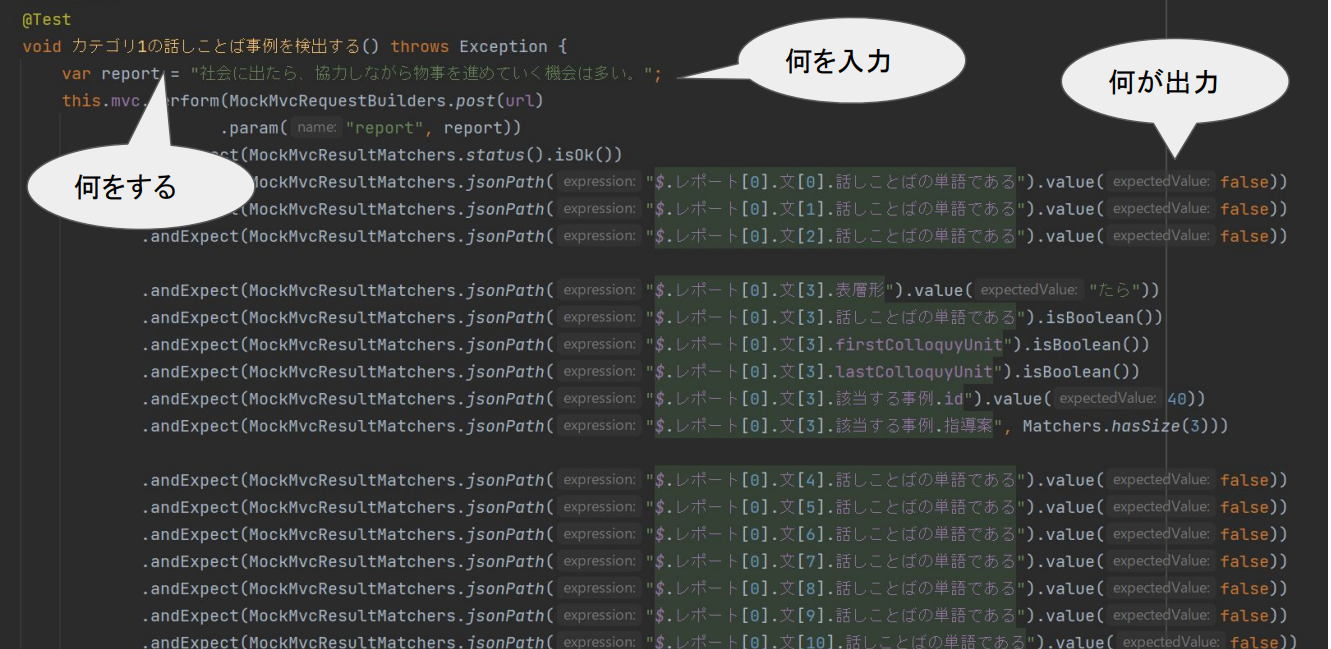
\includegraphics[width=1\linewidth]{image/kaizen3.png}
\caption{テストコードの例}
\label{fig:enter-label}
\end{figure}
\chapter{評価方法の検討}
\section{評価方法}
\subsection{責務を分けたコード}
責務を分けたコードとなっているか、凝集度を用いた定量評価を行う。凝集度とは
凝集度を計測できるツールとしてYegor Bugayenkoが公開jPeekで5つの指標で計測。
\subsection{共有されたメンタルモデルを反映させたコード}
プログラムコードを文書化したものを用いてドメインエキスパートにインタビューを行う定性評価。ユースケース図のプラグインを利用。ライフラインと同期内容を「で」で繋げる形で作成。
\subsection{観察可能な振る舞いを確認できるコード}
テストコードを文書化したものを用いてドメインエキスパートにインタビューを行う定性評価。テスト名とassertの入力・期待する出力を並べる形で作成。
\section{評価結果と考察}
\subsection{責務を分けたコード}
\subsection{共有されたメンタルモデルを反映させたコード}
\subsection{観察可能な振る舞いを確認できるコード}
\chapter{結論}
\section{まとめ}
複雑さの防止効果が高いシステム開発上の要素が判明した。また、その要素がプログラムコードに反映されているか評価する方法について、責務を分けたコードに関しては凝集度による評価、共有されたメンタルモデルを反映させたコードと観察可能な振る舞いを確認できるコードについてはプログラムコードをドキュメント化したものを用いてのインタビューにより評価できることが明らかになった。これにより、責務が分けられたコードであるか誰もが確認できる方法、メンタルモデルや観察可能な振る舞いを誰もが共有できる方法を実現できる可能性が見えたといえる。
\section{今後の課題}
\renewcommand{\bibname}{参考文献}
\addcontentsline{toc}{chapter}{参考文献}
\begin{thebibliography}{10}
\bibitem{haikei}「認知負荷を減らしたプログラミング学習支援に関する研究」石井 元規, 松本 慎平, 林 雄介, 平嶋 宗, 教育システム情報学会 2016年度学生研究発表会, 175-176
\end{thebibliography}

\chapter*{謝辞}
\addcontentsline{toc}{chapter}{謝辞}
\end{document}
